
\documentclass[table,dvipsnames]{beamer}
\mode<presentation>{
	\usetheme{Madrid}
	\setbeamercolor{title}{fg=Black,bg=Blue!15}
	\setbeamercolor{frametitle}{fg=Black,bg=Blue!15}
	\setbeamercolor{block title}{fg=Black,bg=Blue!15}
	\setbeamercolor{block}{fg=Black,bg=Blue!10}
}

\usepackage{default}
\usepackage{graphicx}
\usepackage{booktabs}
\usepackage{xcolor}
\usepackage{multirow}

\title[STM32 Beginner Guide]{Pengenalan Multithreading dan interfacing STM32}
\author{}
\institute[Achmadi ST MT]{
	Institut Teknologi Sepuluh November  \\
	\vspace{10pt}
	FTITOS
	\vspace{10pt}
	CodeDirect
	\medskip
	\textit{}
}
\date{}

\begin{document}
	
	\section{Start}
	
	\begin{frame}
	\titlepage
	\end{frame}

	\section{STM32}
	\subsection{Chip STM32}
	\begin{frame}
		\frametitle{Produk Chip STM32}
		\begin{block}{}
			Chip STM32 adalah microcontroller yang diproduksi ST Microelectronic.
		\end{block}
	
		\begin{block}{}
			Menggunakan arsitektur 32-bit ARM Cortex M0/M3/M4.
		\end{block}
	
		\begin{block}{}
			Standar Industri, tersedia tools dan compiler/toolchain untuk development.
		\end{block}
		\begin{center}
			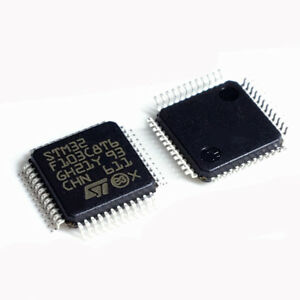
\includegraphics[width=150pt]{images/stm32f103c8}
		\end{center}
	\end{frame}

	\subsection{Board Discovery}
	\begin{frame}
		\frametitle{STM32 Discovery}
		\begin{block}{}
			ST menyediakan beberapa macam board untuk belajar pemula maupun pengembangan awal.
		\end{block}
		
		\begin{center}
			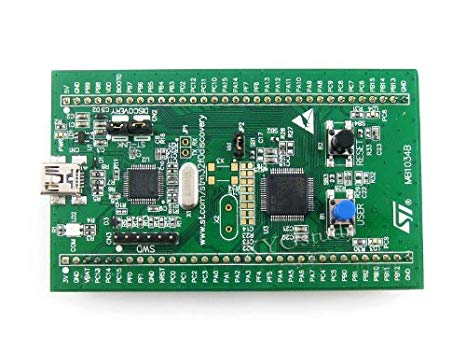
\includegraphics[width=150pt]{images/f0disco}
			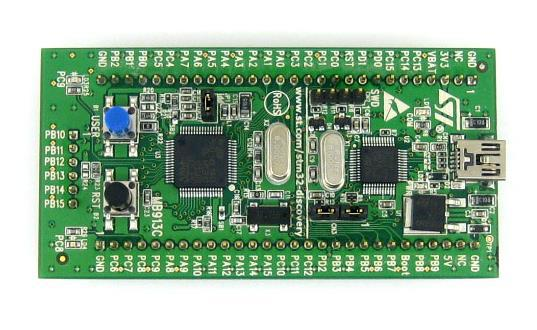
\includegraphics[width=150pt]{images/f1disco}
		\end{center}
	\end{frame}

	\begin{frame}
		\frametitle{STM32 Discovery}
		
		\begin{block}{}
			Tersedia board Discovery untuk seri STM32F0, STM32F1, STM32F2, STM32F3, dan STM32F4.
		\end{block}
		
		\begin{center}
			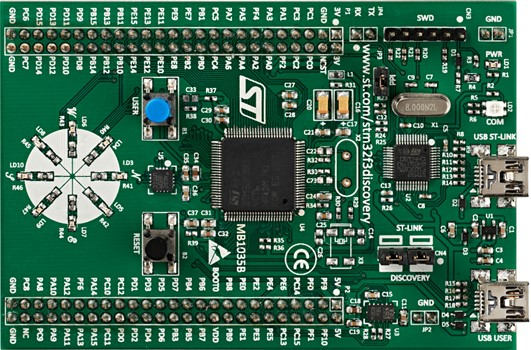
\includegraphics[width=125pt]{images/f3disco}
			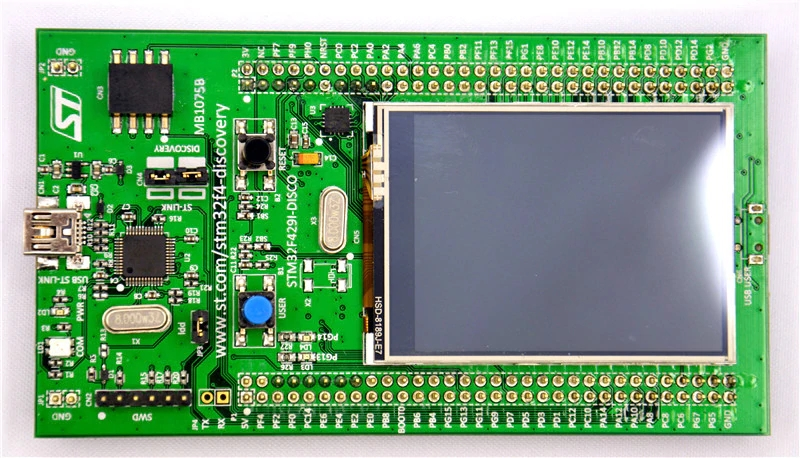
\includegraphics[width=150pt]{images/f4disco}
		\end{center}
	\end{frame}

	\subsection{Nucleo Discovery}
	\begin{frame}
		\frametitle{STM32 Nucleo}
		\begin{block}{}
			Selain Discovery, ST juga menyediakan board Nucleo yang memiliki pin-header layout
			kompatibel dengan Arduino.
		\end{block}
		
		\begin{center}
			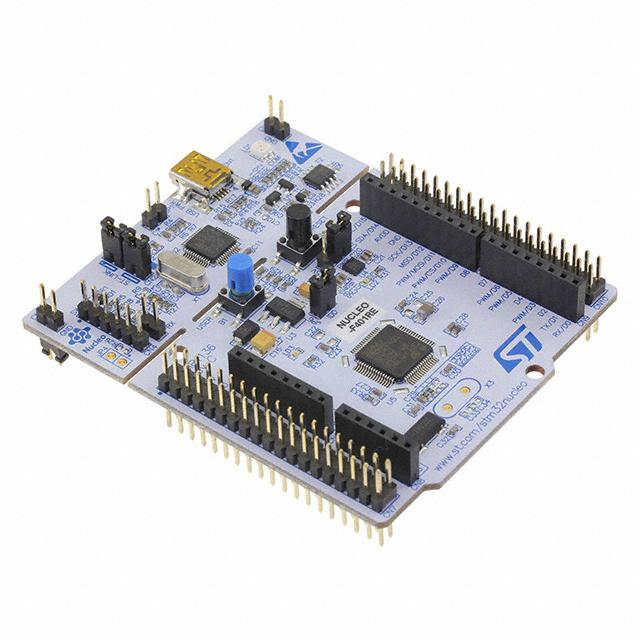
\includegraphics[width=200pt]{images/nucleo}
		\end{center}
	\end{frame}

	\subsection{Unofficial Board}
	\begin{frame}
		\frametitle{STM32 Unofficial Board}
		\begin{block}{}
			Selain Discovery dan Nucleo, tersedia juga board STM32 yang bukan dibuat oleh ST.
		\end{block}
		
		\begin{center}
			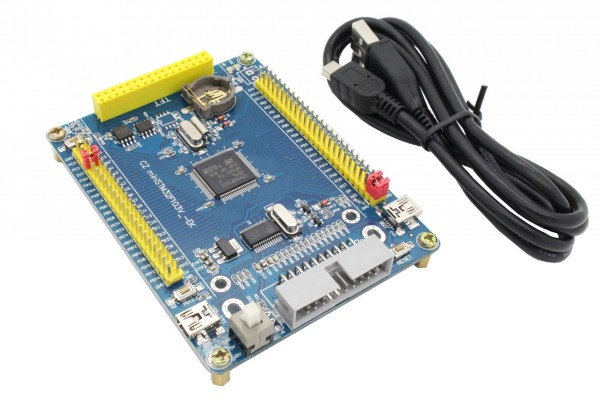
\includegraphics[width=150pt]{images/czmini}
			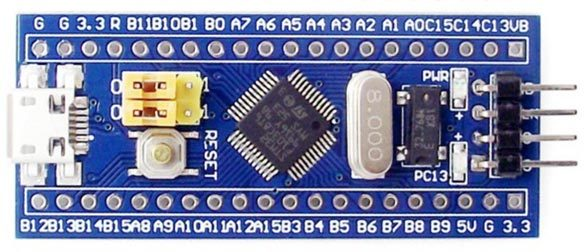
\includegraphics[width=150pt]{images/bluepill}
		\end{center}
	\end{frame}

	\section{Instalasi}
	\subsection{Driver}
	\begin{frame}
		\frametitle{Instalasi Driver}
		\begin{block}{}
			Install driver USB-TTL PL2303, ada di berkas \textbf{installer$\backslash$driver$\backslash$pl2303\_usb\_ttl.zip}
		\end{block}
	
		\begin{block}{}
			Untuk Windows 10 mungkin perlu update dan memilih versi driver secara manual dengan opsi
			\textit{Let me pick a list of available driver on my computer}.
		\end{block}
	
		\begin{block}{}
			Setelah instalasi driver PL2303, cek Device Manager untuk mengetahui nomor COM port
		\end{block}
	
		\begin{center}
			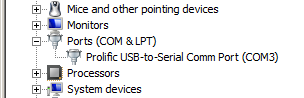
\includegraphics[width=175pt]{images/comport}
		\end{center}
	\end{frame}
	
	\subsection{Development Tools}
	\begin{frame}
		\frametitle{Compiler/Toolchain}
		\begin{block}{}
			\begin{itemize}
				\item Ekstrak file \textbf{STM32\_DevTools.zip} ke alamat semisal \textbf{C:$\backslash$}.
				\item Salin alamat folder binary compiler, semisal \textbf{C:$\backslash$STM32\_DevTools$\backslash$arm-gcc-suite$\backslash$bin}
				\item Masukkan alamatnya ke \textit{Environment Variabels}.
				\begin{itemize}
					\item Buka \textit{Computer} $\rightarrow$ \textit{Properties} $\rightarrow$ \textit{Advanced System Settings}
					\item Klik \textit{Environment Variables}
					\item Klik \textit{Path} yang ada dikolom \textit{System Variables}.
					\item Masukkan alamat tersebut (pisah dengan tanda koma).
				\end{itemize}
			\end{itemize}
		\end{block}
	
		\begin{center}
			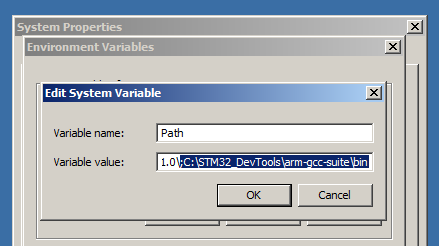
\includegraphics[width=150pt]{images/envar}
		\end{center}
	\end{frame}

	\begin{frame}
		\frametitle{Programmer Notepad}
		\begin{block}{}
			\begin{itemize}
				\item Buka Folder \textbf{STM32\_DevTools$\backslash$programmer-notepad}
				\item Jalankan program \textbf{programmer-notepad.exe} dengan \textit{Run as Administrator}.
				\item Programmer Notepad digunakan untuk kompilasi \textit{sourcecode} ke binary yang siap didownload ke STM32.
			\end{itemize}
		\end{block}
		
		\begin{center}
			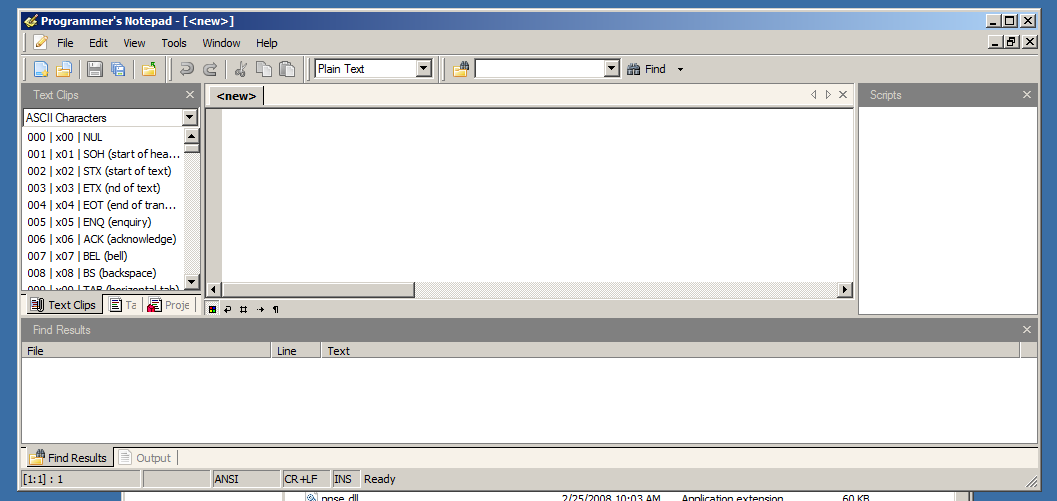
\includegraphics[width=250pt]{images/pn}
		\end{center}
	\end{frame}

	\begin{frame}
	\frametitle{Tes Example}
	\begin{block}{}
		\begin{itemize}
			\item Ekstrak \textbf{ChibiOS\_STM32.zip}.
			\item Buka dengan Programmer Notepad berkas Makefile di folder \textbf{ChibiOS\_STM32$\backslash$example$\backslash$BLUEPILL-BLINK}.
			\item Untuk kompilasi, klik \textit{Tools} $\rightarrow$ \textit{Make All}
		\end{itemize}
	\end{block}
	
	\begin{center}
		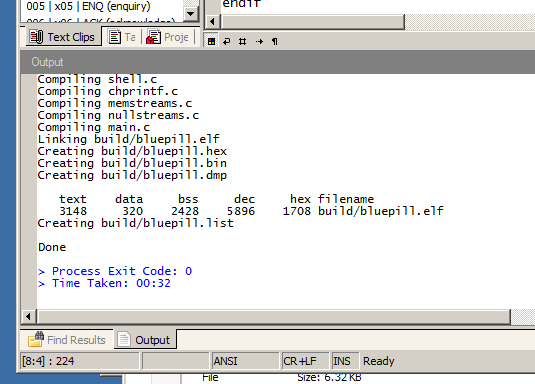
\includegraphics[width=200pt]{images/compile}
	\end{center}
	\end{frame}

	\subsection{Flashloader}
	\begin{frame}
	\frametitle{STM32 bootloader}
		\begin{block}{}
			Saat running $\rightarrow$ Main Flash Memory
		\end{block}
		\begin{block}{}
			Saat programming $\rightarrow$ System Memory
		\end{block}
		
		\begin{center}
			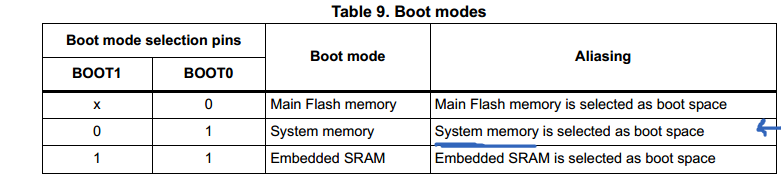
\includegraphics[width=300pt]{images/bootloader}
		\end{center}
	\end{frame}

	\begin{frame}
		\frametitle{UART Line}
		\begin{block}{}
			Sambungan STM32 ke PL2303 (USB-Serial TTL)
			\begin{itemize}
				\item STM32 5v $\rightarrow$ PL2303 5v
				\item STM32 GND $\rightarrow$ PL2303 GND
				\item STM32 TX (PA9) $\rightarrow$ PL2303 RX
				\item STM32 RX (PA10) $\rightarrow$ PL2303 TX
			\end{itemize}
		\end{block}
	
		\begin{block}{}
			\textbf{WARNING}: Jangan sambungkan STM32 3v3 pin ke 5v.
			Maximal toleransi tegangan VDD STM32 hanya sampai 3.6 volt.
		\end{block}
	\end{frame}
	
	\begin{frame}
		\frametitle{Aktivasi bootloader}
		\begin{block}{}
			Aktifkan bootloader untuk untuk masuk mode programming.
			\begin{itemize}
				\item pindahkan jumper \textbf{boot0} ke logic 1.
				\item jumper \textbf{boot1} tetap di logic 0.
				\item tekan reset
			\end{itemize}
		\end{block}
		
		\begin{center}
			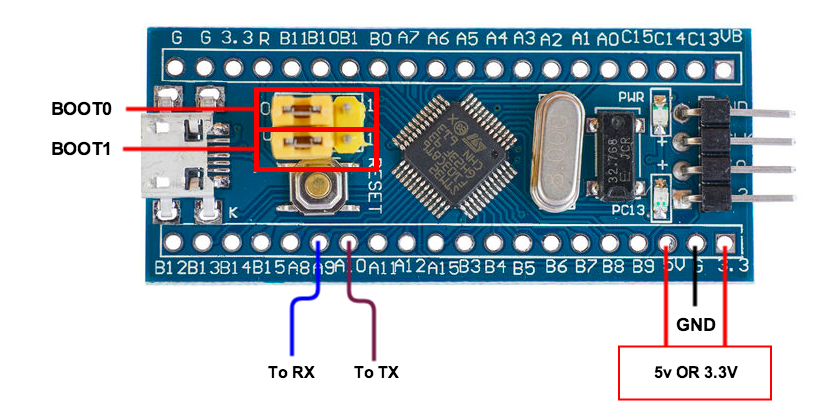
\includegraphics[width=300pt]{images/flashing}
		\end{center}
	\end{frame}

	\subsection{Demonstrator}
	\begin{frame}
		\frametitle{Installasi}
		\begin{block}{}
			Demonstrator adalah program sederhana untuk download binary ke chip STM32 dengan bantuan internal bootloader via UART-Line.
			\begin{itemize}
				\item Install program Demonstrator yang ada di \textbf{installer$\backslash$tools$\backslash$stm32\_flasher.zip}
				\item Jalankan Demonstator GUI dari menu dengan \textit{Run as Administrator}.
				\item Pastikan nomor COM port sesuai dengan nomor serial port PL2302 di Device Manager.
			\end{itemize}
		\end{block}
		
		\begin{center}
			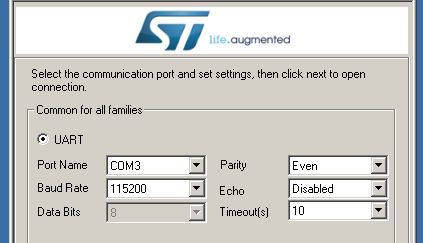
\includegraphics[width=150pt]{images/demons}
		\end{center}
	\end{frame}

	\subsection{Downloading}
	\begin{frame}
		\frametitle{Next}
		\begin{block}{}
			Klik \textit{Next}. Jika ada pesan error, cek wiring, kondisi jumper boot, dan tekan reset lagi.
		\end{block}
		\begin{center}
			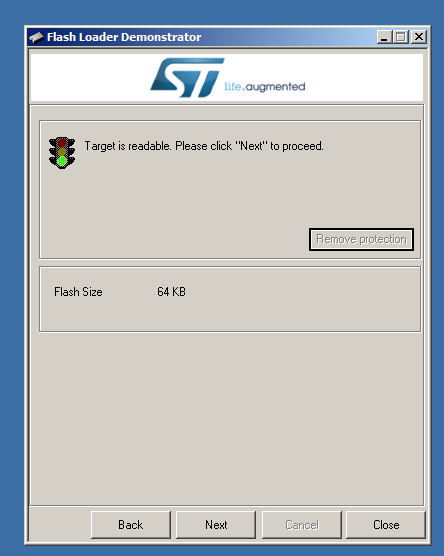
\includegraphics[width=150pt]{images/demons1}
			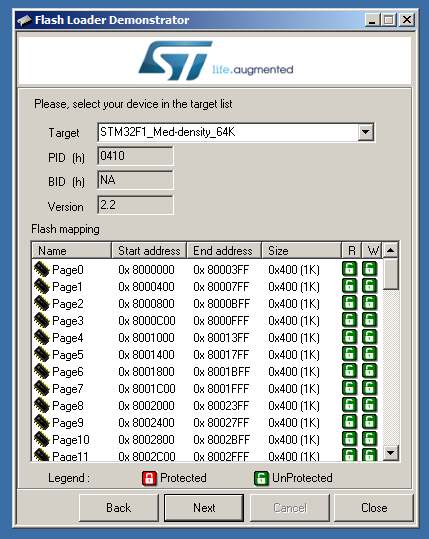
\includegraphics[width=150pt]{images/demons2}
		\end{center}
	\end{frame}

	\begin{frame}
		\frametitle{Download binary}
		\begin{block}{}
			\begin{itemize}
				\item pilih \textit{Download to Device}
				\item isi alamat file yang akan di download:
				\begin{itemize}
					\item Klik browser (simbol tiga titik) disebelah address bar
					\item Di open file dialog, pilih tipe file \textbf{*.bin} atau \textbf{*.hex}
					\item Cari file yanga akan didownload ke chip, sebagai contoh disini:\\
					\textbf{ChibiOS\_STM32$\backslash$example$\backslash$BLUEPILL-BLINK$\backslash$build$\backslash$bluepill.bin}.
				\end{itemize}
				\item Klik \textit{Global Erase}.
				\item Centang \textit{Verify after download}.
			\end{itemize}
		\end{block}
		\begin{center}
			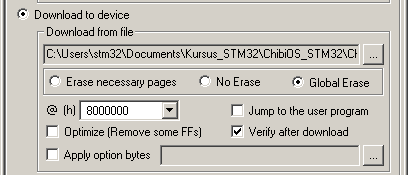
\includegraphics[width=200pt]{images/demons3}
		\end{center}
	\end{frame}

	\begin{frame}
		\frametitle{Download Success}
		\begin{block}{}
			Tunggu proses Downloading selesai dan sukses.
			Program Demonstrator bisa di \textit{Close}.
		\end{block}
		\begin{center}
			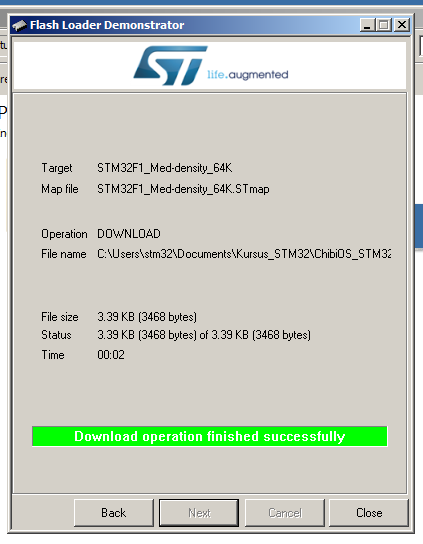
\includegraphics[width=150pt]{images/demons4}
		\end{center}
	\end{frame}

	\begin{frame}
		\frametitle{Aktivasi Main Program}
		\begin{block}{}
			Aktivasi Main program untuk untuk masuk mode running.
			\begin{itemize}
				\item pindahkan jumper \textbf{boot0} ke logic 0.
				\item jumper \textbf{boot1} tetap di logic 0.
				\item tekan reset
			\end{itemize}
		\end{block}
		
		\begin{center}
			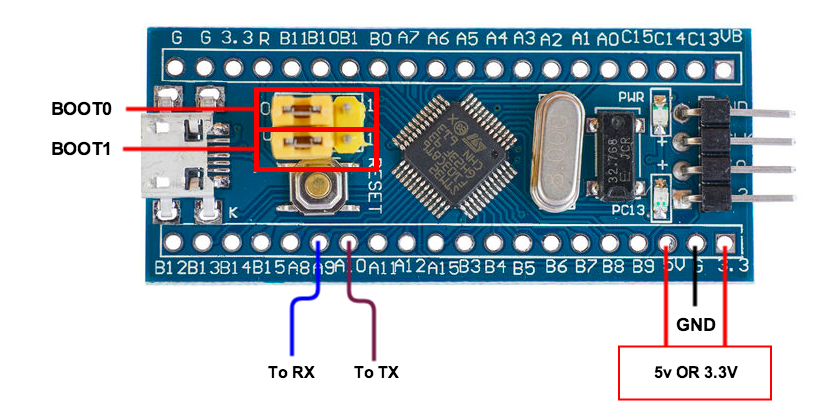
\includegraphics[width=300pt]{images/flashing}
		\end{center}
	\end{frame}

\end{document}
